\chaptercustom{3}{MÔ HÌNH HỆ THỐNG VÀ TRIỂN KHAI MÔ PHỎNG}
\setcounter{section}{3}
\label{chap:system_simulation}

\subsection{Cấu hình kênh MIMO băng rộng}
\label{subsec:ch3_mimo_configuration}

Chương 2 đã phân tích cơ sở lý thuyết của biểu diễn DPS đối với tín hiệu giới hạn băng trên khối hữu hạn. Chương này chuyển phần lý thuyết đó thành một mô hình kênh và một quy trình mô phỏng cụ thể. Trình tự trình bày gồm bốn bước: mô tả ý nghĩa vật lý của kênh MIMO băng rộng; lấy mẫu kênh theo bốn chiều; xây dựng cơ sở DPS từ miền giới hạn băng; và triển khai các nhánh so sánh trong MATLAB. Nhờ đó, mỗi ký hiệu toán học đều có thể đối chiếu với một đại lượng vật lý hoặc một biến trong chương trình.

Xét hệ thống MIMO băng rộng gồm \(N_{\mathrm{Tx}}\) anten phát và \(N_{\mathrm{Rx}}\) anten thu. Mỗi cặp anten phát--thu tạo thành một kênh con; do đó, đáp ứng của toàn hệ thống phải mô tả đồng thời nhiều kênh con thay vì chỉ một tín hiệu vô tuyến. Các anten được giả thiết tạo thành mảng tuyến tính đều (Uniform Linear Array, ULA) với khoảng cách chuẩn hóa \(D_s/\lambda=0{,}5\), trong đó \(D_s\) là khoảng cách giữa hai phần tử anten liên tiếp và \(\lambda\) là bước sóng sóng mang.

Đáp ứng kênh được mô hình hóa theo GCM, trong đó tín hiệu từ máy phát đến máy thu qua nhiều đường truyền do phản xạ hoặc tán xạ. Mỗi đường được biểu diễn bằng một MPC. MPC thứ \(p\) có trọng số phức \(\eta_p\), dịch Doppler \(\omega_p\), trễ \(\tau_p\), góc khởi hành \(\phi_p\) và góc tới \(\psi_p\). Trọng số \(\eta_p\) chứa cả biên độ và pha ban đầu của đường truyền; bốn đại lượng còn lại quyết định sự thay đổi pha theo thời gian, tần số và vị trí anten.

Theo mô hình trong bài báo Kaltenberger và cộng sự, đáp ứng kênh phụ thuộc đồng thời vào thời gian \(t\), tần số khảo sát \(f\), vị trí anten phát \(x\) và vị trí anten thu \(y\) \cite{Kaltenberger2007}. Ở đây, \(f\) là vị trí tần số trong băng tín hiệu, không phải tần số sóng mang \(f_c\).

Hình~\ref{fig:ch3_gcm_mimo} minh họa cách GCM mô tả kênh MIMO thông qua các đường truyền trực tiếp hoặc phản xạ qua các vật tán xạ. Trong mỗi đường truyền, góc khởi hành tại phía phát và góc tới tại phía thu quyết định thành phần pha không gian của MPC tương ứng.

\begin{figure}[H]
    \centering
    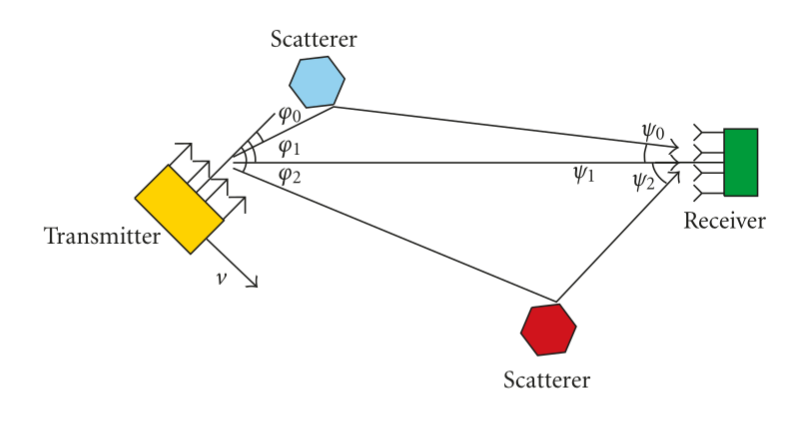
\includegraphics[width=0.82\textwidth]{results/figures/gcm_MIMO.png}
    \caption{Minh họa mô hình kênh MIMO dựa trên hình học với các thành phần đa đường}
    \label{fig:ch3_gcm_mimo}
\end{figure}

Trong mô hình toán học, mỗi đường truyền trong Hình~\ref{fig:ch3_gcm_mimo} được biểu diễn bằng một MPC có trọng số phức, dịch Doppler, trễ truyền lan và hai góc không gian. Tổng đóng góp của các MPC tạo thành đáp ứng kênh liên tục:
\begin{equation}
h(t,f,x,y)
=
\sum_{p=0}^{P-1}
\eta_p
e^{j2\pi \omega_p t}
e^{-j2\pi \tau_p f}
e^{j\frac{2\pi}{\lambda}\sin(\phi_p)x}
e^{-j\frac{2\pi}{\lambda}\sin(\psi_p)y}.
\label{eq:ch3_continuous_gcm}
\end{equation}
Dấu pha trong \eqref{eq:ch3_continuous_gcm} thể hiện bốn cơ chế vật lý: Doppler theo thời gian, trễ theo tần số, pha không gian ở phía phát và pha không gian ở phía thu. Giá trị \(h(t,f,x,y)\) là một số phức biểu diễn hệ số kênh tại đúng thời điểm, tần số và cặp vị trí anten đang xét. Quy ước dấu này được giữ nhất quán trong mô hình rời rạc và trong hàm MATLAB \texttt{compute\_mimo\_soce}.

\subsection{Rời rạc hóa bốn chiều}
\label{subsec:ch3_discretization}

Để tính kênh trên máy tính, bốn biến liên tục được thay bằng các điểm lấy mẫu
\(t=mT_s\), \(f=qF_s\), \(x=sD_s\) và \(y=rD_s\). Chỉ số thời gian là \(m=0,\ldots,M-1\), chỉ số tần số là \(q=0,\ldots,Q-1\), chỉ số anten phát là \(s=0,\ldots,N_{\mathrm{Tx}}-1\), và chỉ số anten thu là \(r=0,\ldots,N_{\mathrm{Rx}}-1\). Vì vậy, một phần tử \(h_{m,q,s,r}\) là hệ số kênh giữa anten phát \(s\) và anten thu \(r\), tại mẫu thời gian \(m\) và điểm tần số \(q\).

Để số mũ phức chỉ còn phụ thuộc vào các chỉ số nguyên, các tham số vật lý được đổi thành tần số chuẩn hóa:
\begin{equation}
\nu_p = \omega_p T_s,
\quad
\theta_p = \tau_p F_s,
\quad
\zeta_p = \sin(\phi_p)\frac{D_s}{\lambda},
\quad
\xi_p = \sin(\psi_p)\frac{D_s}{\lambda},
\label{eq:ch3_normalized_variables}
\end{equation}
trong đó \(T_s\) là chu kỳ lấy mẫu theo thời gian và \(F_s\) là khoảng cách giữa hai điểm tần số liên tiếp trong mô phỏng. Các đại lượng \(\nu_p,\theta_p,\zeta_p,\xi_p\) không có đơn vị và biểu thị số chu kỳ pha trên một bước chỉ số ở từng chiều.

Thay \eqref{eq:ch3_normalized_variables} vào \eqref{eq:ch3_continuous_gcm}, đáp ứng kênh rời rạc bốn chiều có dạng:
\begin{equation}
h_{m,q,s,r}
=
\sum_{p=0}^{P-1}
\eta_p
e^{j2\pi(\nu_p m-\theta_p q+\zeta_p s-\xi_p r)}.
\label{eq:ch3_discrete_soce}
\end{equation}
Phương trình \eqref{eq:ch3_discrete_soce} cho thấy tại mỗi bộ chỉ số \((m,q,s,r)\), chương trình phải tính và cộng đóng góp của toàn bộ \(P\) MPC. Đây là SoCE tham chiếu trong mô phỏng. Trong MATLAB, tất cả các giá trị \(h_{m,q,s,r}\) được xếp vào mảng bốn chiều, còn gọi là tensor, \texttt{H\_soce} có kích thước \(M\times Q\times N_{\mathrm{Tx}}\times N_{\mathrm{Rx}}\).

Các tham số MPC trong mô phỏng hiện tại được sinh ngẫu nhiên trong miền giới hạn băng đã định trước. Trọng số \(\eta_p\) được sinh theo phân bố Gauss phức tròn với chuẩn hóa công suất trung bình, còn các tần số chuẩn hóa \(\nu_p,\theta_p,\zeta_p,\xi_p\) được lấy đều trong các khoảng vật lý tương ứng. Các giả thiết này dùng để kiểm tra biểu diễn DPS và không nhằm tái tạo đầy đủ một kịch bản kênh chuẩn cụ thể.

\subsection{Miền giới hạn băng}
\label{subsec:ch3_band_region}

Mặc dù khối kênh có nhiều phần tử, các hàm mũ trong \eqref{eq:ch3_discrete_soce} không thể có tần số tùy ý. Vận tốc cực đại giới hạn Doppler, độ trễ cực đại giới hạn biến thiên theo tần số, còn khoảng góc giới hạn biến thiên theo vị trí anten. Vì vậy, các tần số chuẩn hóa chỉ nằm trong miền:
\begin{equation}
\mathcal{W}
=
\mathcal{W}_t
\times
\mathcal{W}_f
\times
\mathcal{W}_{\mathrm{Tx}}
\times
\mathcal{W}_{\mathrm{Rx}}.
\label{eq:ch3_band_region}
\end{equation}
Trong script MATLAB, các miền thành phần được xác định bởi:
\begin{equation}
\mathcal{W}_t=[-\nu_{\mathrm{D,max}},\nu_{\mathrm{D,max}}],
\quad
\mathcal{W}_f=[-\theta_{\max},0],
\label{eq:ch3_time_frequency_bands}
\end{equation}
và:
\begin{equation}
\mathcal{W}_{\mathrm{Tx}}=[\zeta_{\min},\zeta_{\max}],
\quad
\mathcal{W}_{\mathrm{Rx}}=[-\xi_{\max},-\xi_{\min}].
\label{eq:ch3_spatial_bands}
\end{equation}
Trong đó:
\begin{equation}
\nu_{\mathrm{D,max}}
=
\frac{v_{\max} f_c T_s}{c},
\quad
\theta_{\max}=\tau_{\max}F_s.
\label{eq:ch3_doppler_delay_bounds}
\end{equation}
Các giới hạn không gian được tính từ khoảng góc tới và góc khởi hành:
\begin{equation}
\zeta_{\min,\max}=\sin(\phi_{\min,\max})\frac{D_s}{\lambda},
\quad
\xi_{\min,\max}=\sin(\psi_{\min,\max})\frac{D_s}{\lambda}.
\label{eq:ch3_spatial_bounds}
\end{equation}

Để tạo cơ sở DPS có thể dịch tâm tần số, mỗi chiều được mô tả bằng tâm băng \(W_0\) và nửa băng thông \(W_{\max}\). Cách ánh xạ trong MATLAB là:
\begin{equation}
\begin{aligned}
&\text{thời gian:}      && W_0=0,\quad W_{\max}=\nu_{\mathrm{D,max}},\\
&\text{tần số:}         && W_0=-\theta_{\max}/2,\quad W_{\max}=\theta_{\max}/2,\\
&\text{không gian phát:}&& W_0=(\zeta_{\min}+\zeta_{\max})/2,\quad
W_{\max}=(\zeta_{\max}-\zeta_{\min})/2,\\
&\text{không gian thu:} && W_0=-(\xi_{\min}+\xi_{\max})/2,\quad
W_{\max}=(\xi_{\max}-\xi_{\min})/2.
\end{aligned}
\label{eq:ch3_dps_band_mapping}
\end{equation}
Các dấu âm ở chiều tần số và chiều thu xuất phát từ dấu pha \(-\theta_p q\) và \(-\xi_p r\) trong \eqref{eq:ch3_discrete_soce}. Việc xác định đúng tâm băng và nửa băng thông là bước nối giữa mô hình vật lý với cơ sở DPS: cơ sở chỉ biểu diễn tốt kênh khi miền băng dùng để tạo cơ sở bao phủ các tần số của MPC.

\subsection{Cơ sở DPS đa chiều}
\label{subsec:ch3_multidim_dps}

Với miền giới hạn băng dạng tích Descartes trong \eqref{eq:ch3_band_region}, mỗi chiều có thể dùng một cơ sở DPS riêng. Gọi \(\mathbf{V}_t\), \(\mathbf{V}_f\), \(\mathbf{V}_{\mathrm{Tx}}\) và \(\mathbf{V}_{\mathrm{Rx}}\) lần lượt là các ma trận cơ sở DPS theo thời gian, tần số, anten phát và anten thu. Mỗi cột của một ma trận là một vector cơ sở; chẳng hạn, \(v^{(t)}_{d_t}[m]\) là giá trị của vector DPS thứ \(d_t\) tại mẫu thời gian \(m\).

Ý tưởng tái tạo là thay tổng theo các MPC trong \eqref{eq:ch3_discrete_soce} bằng tổng theo một số hữu hạn các hàm cơ sở. Hệ số \(\alpha_{d_t,d_f,d_{\mathrm{Tx}},d_{\mathrm{Rx}}}\) cho biết mức đóng góp của một tổ hợp gồm bốn vector cơ sở. Khi đó, xấp xỉ DPS bốn chiều có thể viết:
\begin{equation}
\hat{h}_{m,q,s,r}
=
\sum_{d_t=0}^{D_t-1}
\sum_{d_f=0}^{D_f-1}
\sum_{d_{\mathrm{Tx}}=0}^{D_{\mathrm{Tx}}-1}
\sum_{d_{\mathrm{Rx}}=0}^{D_{\mathrm{Rx}}-1}
\alpha_{d_t,d_f,d_{\mathrm{Tx}},d_{\mathrm{Rx}}}
v^{(t)}_{d_t}[m]
v^{(f)}_{d_f}[q]
v^{(\mathrm{Tx})}_{d_{\mathrm{Tx}}}[s]
v^{(\mathrm{Rx})}_{d_{\mathrm{Rx}}}[r].
\label{eq:ch3_4d_dps_reconstruction}
\end{equation}
Số hệ số của biểu diễn này là:
\begin{equation}
D_{\mathrm{total}}
=D_tD_fD_{\mathrm{Tx}}D_{\mathrm{Rx}}.
\label{eq:ch3_total_dps_dimension}
\end{equation}

Trong script, số vector DPS của từng chiều được chọn theo số chiều thiết yếu cộng thêm một số vector dự phòng:
\begin{equation}
\begin{aligned}
D_t  &= \left\lceil 2\nu_{\mathrm{D,max}}M \right\rceil + 1 + G,\\
D_f  &= \left\lceil \theta_{\max}Q \right\rceil + 1 + G,\\
D_{\mathrm{Tx}} &= \left\lceil (\zeta_{\max}-\zeta_{\min})N_{\mathrm{Tx}} \right\rceil + 1 + G,\\
D_{\mathrm{Rx}} &= \left\lceil (\xi_{\max}-\xi_{\min})N_{\mathrm{Rx}} \right\rceil + 1 + G.
\end{aligned}
\label{eq:ch3_dps_dimension_rule}
\end{equation}
Trong mô phỏng hiện tại, \(G=4\). Số hạng dự phòng này giữ thêm các vector ở rìa không gian con nhằm giảm sai số cắt. Các giá trị \(D_t,D_f,D_{\mathrm{Tx}},D_{\mathrm{Rx}}\) sau đó được chặn trên bởi số mẫu tương ứng của từng chiều, vì một chiều có \(N\) mẫu không thể có hơn \(N\) vector cơ sở độc lập. Quy tắc trên là giả thiết thiết kế của mô phỏng hiện tại, chưa phải thủ tục tự động chọn số chiều từ một ngưỡng sai số cho trước.

\subsection{Các nhánh mô phỏng MATLAB}
\label{subsec:ch3_simulation_branches}

Phiên bản mô phỏng xấp xỉ triển khai bốn nhánh chính trên cùng một tập MPC. Nhánh thứ nhất là SoCE tham chiếu, trong đó chương trình tính trực tiếp \eqref{eq:ch3_discrete_soce}. Ba nhánh còn lại không thay đổi kịch bản truyền sóng mà chỉ thay đổi cách biểu diễn và tái tạo cùng một kênh. Vì vậy, sai khác giữa chúng với SoCE phản ánh sai số của biểu diễn DPS trong cấu hình đang xét.

Nhánh thứ hai là DPS chính xác. Với mỗi MPC, script tạo các vector hàm mũ theo bốn chiều và chiếu chính xác lên từng cơ sở DPS:
\begin{equation}
\begin{aligned}
\boldsymbol{\gamma}^{(t)}_p
&=\mathbf{V}_t^{H}\mathbf{e}^{(t)}(\nu_p),&
\boldsymbol{\gamma}^{(f)}_p
&=\mathbf{V}_f^{H}\mathbf{e}^{(f)}(-\theta_p),\\
\boldsymbol{\gamma}^{(\mathrm{Tx})}_p
&=\mathbf{V}_{\mathrm{Tx}}^{H}\mathbf{e}^{(\mathrm{Tx})}(\zeta_p),&
\boldsymbol{\gamma}^{(\mathrm{Rx})}_p
&=\mathbf{V}_{\mathrm{Rx}}^{H}\mathbf{e}^{(\mathrm{Rx})}(-\xi_p).
\end{aligned}
\label{eq:ch3_exact_projection_coefficients}
\end{equation}
Tensor hệ số của toàn bộ kênh được tạo bằng tổng các tích ngoài:
\begin{equation}
\boldsymbol{\alpha}_{\mathrm{exact}}
=
\sum_{p=0}^{P-1}
\eta_p\,
\boldsymbol{\gamma}^{(t)}_p
\circ
\boldsymbol{\gamma}^{(f)}_p
\circ
\boldsymbol{\gamma}^{(\mathrm{Tx})}_p
\circ
\boldsymbol{\gamma}^{(\mathrm{Rx})}_p.
\label{eq:ch3_exact_alpha}
\end{equation}
Ký hiệu \(\circ\) trong \eqref{eq:ch3_exact_alpha} là tích ngoài: bốn vector hệ số một chiều được ghép thành một tensor hệ số bốn chiều. Nhánh này dùng để đánh giá chất lượng của không gian con DPS đã chọn. Tên gọi ``DPS chính xác'' chỉ có nghĩa các hệ số chiếu được tính bằng tích vô hướng chính xác; kênh tái tạo vẫn có thể sai khác với SoCE do chỉ giữ một số hữu hạn vector DPS.

Nhánh thứ ba là DPS xấp xỉ 4D. Thay vì tạo toàn bộ vector hàm mũ rồi tính tích vô hướng như \eqref{eq:ch3_exact_projection_coefficients}, chương trình dùng hàm \texttt{approximate\_gamma\_1d(...)} để ước lượng trực tiếp hệ số một chiều từ vị trí tần số chuẩn hóa của MPC trên một cơ sở DPS có độ phân giải cao. Các hệ số này sau đó được ghép bằng tích ngoài giống \eqref{eq:ch3_exact_alpha}. Đây là nhánh kiểm tra việc áp dụng công thức xấp xỉ hàm sóng DPS cho cả bốn chiều.

Nhánh thứ tư là phương pháp hybrid. Nhánh này dùng DPS xấp xỉ cho hai chiều thời gian và tần số, nhưng giữ phần không gian anten dưới dạng hàm mũ trực tiếp:
\begin{equation}
\boldsymbol{\alpha}_{\mathrm{hybrid}}
=
\sum_{p=0}^{P-1}
\eta_p\,
\boldsymbol{\gamma}^{(t)}_p
\circ
\boldsymbol{\gamma}^{(f)}_p
\circ
\mathbf{e}^{(\mathrm{Tx})}(\zeta_p)
\circ
\mathbf{e}^{(\mathrm{Rx})}(-\xi_p).
\label{eq:ch3_hybrid_alpha}
\end{equation}
Trong MATLAB, nhánh này tương ứng với \texttt{build\_alpha\_approx\_hybrid(...)} và \texttt{reconstruct\_hybrid(...)}. Cách triển khai này phù hợp với định hướng thực tế của bài báo: khi số anten không lớn, lợi ích của DPS ở chiều không gian có thể hạn chế, trong khi DPS theo thời gian và tần số vẫn khai thác được cấu trúc giới hạn băng của kênh \cite{Kaltenberger2007}.

\subsection{Tham số và ánh xạ biến MATLAB}
\label{subsec:ch3_matlab_mapping}

Bảng~\ref{tab:ch3_simulation_parameters} tóm tắt các tham số chính đang dùng trong script mô phỏng. Đây là các tham số cấu hình, không phải kết quả đánh giá hiệu năng.

\begin{table}[H]
    \centering
    \small
    \caption{Tham số mô phỏng chính trong script MATLAB}
    \label{tab:ch3_simulation_parameters}
    \begin{tabularx}{\textwidth}{l l X}
        \toprule
        Ký hiệu & Biến MATLAB & Giá trị trong mô phỏng hiện tại \\
        \midrule
        \(f_c\) & \texttt{fc} & \(2\,\mathrm{GHz}\) \\
        \(v_{\max}\) & \texttt{vmax} & \(100/3{,}6\,\mathrm{m/s}\) \\
        \(T_s\) & \texttt{Ts} & \(1/3{,}84\,\mathrm{MHz}\) \\
        \(F_s\) & \texttt{Fbin} & \(15\,\mathrm{kHz}\) \\
        \(\tau_{\max}\) & \texttt{tau\_max} & \(3{,}7\,\mu\mathrm{s}\) \\
        \(D_s/\lambda\) & \texttt{d\_over\_lambda} & \(0{,}5\) \\
        \([\phi_{\min},\phi_{\max}]\) & \texttt{phi\_min}, \texttt{phi\_max} & \([-5^\circ,5^\circ]\) \\
        \([\psi_{\min},\psi_{\max}]\) & \texttt{psi\_min}, \texttt{psi\_max} & \([-5^\circ,5^\circ]\) \\
        \(M,Q\) & \texttt{M}, \texttt{Q} & \(256,64\) \\
        \(N_{\mathrm{Tx}},N_{\mathrm{Rx}}\) & \texttt{N\_Tx}, \texttt{N\_Rx} & \(4,4\) \\
        \(P\) & \texttt{P} & \(80\) \\
        \bottomrule
    \end{tabularx}
\end{table}

Bảng~\ref{tab:ch3_variable_mapping} trình bày ánh xạ giữa ký hiệu trong chương và biến MATLAB. Việc thống nhất ánh xạ này giúp đảm bảo các phương trình trong đồ án và mã mô phỏng sử dụng cùng quy ước dấu pha.

\begin{table}[H]
    \centering
    \small
    \caption{Ánh xạ ký hiệu mô hình với biến MATLAB}
    \label{tab:ch3_variable_mapping}
    \begin{tabularx}{\textwidth}{l l X}
        \toprule
        Ký hiệu & Biến MATLAB & Ý nghĩa \\
        \midrule
        \(h_{m,q,s,r}\) & \texttt{H\_soce} & Kênh SoCE tham chiếu \\
        \(\hat{h}_{m,q,s,r}\) & \texttt{H\_exact}, \texttt{H\_approx\_4d}, \texttt{H\_hybrid} & Kênh tái tạo từ các nhánh DPS \\
        \(\eta_p\) & \texttt{eta(p)} & Trọng số phức của MPC thứ \(p\) \\
        \(\nu_p\) & \texttt{nu(p)} & Dịch Doppler chuẩn hóa \\
        \(\theta_p\) & \texttt{theta(p)} & Trễ chuẩn hóa theo tần số \\
        \(\zeta_p\) & \texttt{zeta(p)} & Tần số không gian phía phát \\
        \(\xi_p\) & \texttt{xi(p)} & Tần số không gian phía thu \\
        \(\mathbf{V}_t,\mathbf{V}_f\) & \texttt{dim\_t.V}, \texttt{dim\_f.V} & Cơ sở DPS theo thời gian và tần số \\
        \(\mathbf{V}_{\mathrm{Tx}},\mathbf{V}_{\mathrm{Rx}}\) & \texttt{dim\_tx.V}, \texttt{dim\_rx.V} & Cơ sở DPS theo không gian phát và thu \\
        \(\boldsymbol{\alpha}_{\mathrm{exact}}\) & \texttt{alpha\_exact} & Hệ số DPS chiếu chính xác \\
        \(\boldsymbol{\alpha}_{\mathrm{approx}}\) & \texttt{alpha\_approx\_4d} & Hệ số DPS xấp xỉ 4D \\
        \(\boldsymbol{\alpha}_{\mathrm{hybrid}}\) & \texttt{alpha\_hybrid} & Hệ số phương pháp hybrid \\
        \bottomrule
    \end{tabularx}
\end{table}

\subsection{Quy trình mô phỏng}
\label{subsec:ch3_simulation_flow}

Quy trình mô phỏng trong MATLAB gồm các bước chính sau. Đầu tiên, chương trình thiết lập seed bằng \texttt{rng(1)} để bảo đảm khả năng tái lập. Tiếp theo, chương trình thiết lập tham số vật lý, sinh \(P\) MPC trong miền giới hạn băng và tạo các cơ sở DPS một chiều. Sau đó, kênh SoCE tham chiếu được tính theo \eqref{eq:ch3_discrete_soce}.

Hình~\ref{fig:ch3_simulation_flowchart} tóm tắt luồng xử lý chính của mô phỏng. Sơ đồ cho thấy SoCE được dùng làm nhánh tham chiếu, trong khi ba nhánh DPS được tính song song về mặt thuật toán trước khi so sánh sai số và thời gian chạy.

\begin{figure}[H]
    \centering
    \begin{tikzpicture}[
        block/.style={draw, rounded corners=2pt, align=center, text width=3.4cm, minimum height=0.95cm, font=\small},
        branch/.style={draw, rounded corners=2pt, align=center, text width=3.1cm, minimum height=1.1cm, font=\scriptsize},
        arrow/.style={->, thick}
    ]
        \node[block] (init) at (0,0) {Thiết lập seed và tham số mô phỏng};
        \node[block] (mpc) at (0,-1.55) {Sinh MPC trong miền giới hạn băng};
        \node[block] (basis) at (0,-3.10) {Tạo cơ sở DPS một chiều};
        \node[block] (soce) at (0,-4.65) {Tính kênh SoCE tham chiếu};

        \node[branch] (exact) at (-4.1,-6.35) {DPS chính xác\\Tính \(\boldsymbol{\alpha}_{\mathrm{exact}}\)};
        \node[branch] (approx) at (0,-6.35) {DPS xấp xỉ 4D\\Tính \(\boldsymbol{\alpha}_{\mathrm{approx}}\)};
        \node[branch] (hybrid) at (4.1,-6.35) {Phương pháp hybrid\\Tính \(\boldsymbol{\alpha}_{\mathrm{hybrid}}\)};

        \node[branch] (rexact) at (-4.1,-8.10) {Tái tạo\\\(\hat{H}_{\mathrm{exact}}\)};
        \node[branch] (rapprox) at (0,-8.10) {Tái tạo\\\(\hat{H}_{\mathrm{approx}}\)};
        \node[branch] (rhybrid) at (4.1,-8.10) {Tái tạo\\\(\hat{H}_{\mathrm{hybrid}}\)};

        \node[block, text width=4.2cm] (metrics) at (0,-9.95) {Tính MSE, NMSE, sai số cực đại và thời gian chạy};
        \node[block, text width=4.2cm] (outputs) at (0,-12.00) {Tạo hình và bảng phục vụ phân tích kết quả};

        \draw[arrow] (init) -- (mpc);
        \draw[arrow] (mpc) -- (basis);
        \draw[arrow] (basis) -- (soce);
        \draw[arrow] (soce) -- (exact);
        \draw[arrow] (soce) -- (approx);
        \draw[arrow] (soce) -- (hybrid);
        \draw[arrow] (exact) -- (rexact);
        \draw[arrow] (approx) -- (rapprox);
        \draw[arrow] (hybrid) -- (rhybrid);
        \draw[arrow] (rexact) -- (metrics);
        \draw[arrow] (rapprox) -- (metrics);
        \draw[arrow] (rhybrid) -- (metrics);
        \draw[arrow] (soce.east) -- ++(6.0,0) |- (metrics.east);
        \draw[arrow] (metrics) -- (outputs);
    \end{tikzpicture}
    \caption{Quy trình mô phỏng và đánh giá các nhánh biểu diễn kênh}
    \label{fig:ch3_simulation_flowchart}
\end{figure}

Sau khi có kênh tham chiếu, chương trình lần lượt tính hệ số cho ba nhánh DPS: chiếu chính xác, xấp xỉ 4D và phương pháp hybrid. Các tensor hệ số được tái tạo bằng phép nhân tensor theo từng mode thông qua hàm \texttt{mode\_product(...)}. Cuối cùng, chương trình tính các đại lượng sai số và thời gian chạy để phục vụ phần đánh giá ở Chương 4.

\subsection{Kết luận chương}
\label{subsec:ch3_conclusion}

Chương này đã trình bày mô hình GCM MIMO băng rộng, quá trình rời rạc hóa bốn chiều và cách triển khai các nhánh mô phỏng trong MATLAB. SoCE được dùng làm kênh tham chiếu; DPS chính xác dùng để kiểm tra không gian con; DPS xấp xỉ 4D kiểm tra công thức hệ số dựa trên hàm sóng DPS; và phương pháp hybrid kết hợp DPS theo thời gian--tần số với hàm mũ không gian trực tiếp. Cấu trúc này tạo cơ sở cho Chương 4 đánh giá sai số và thời gian tính toán của các nhánh mô phỏng.

\cleardoublepage
